\chapter{Implementácia}

Nasledujúca kapitola sa bude zaoberať popisom implementácie dvoch programov pre snímanie prechodov ľudí cez virtuálnu bránu. Prvý program je založený na základe snímania hĺbkovej mapy pomocov hĺbkomera a druhý  na použití bežnej RGB web kamery.

\section{Programovací jazyk a využité knižnice}
Pri implementácii oboch programov som zvolil programovací jazyk \textit{Python 3} v spojení s knižnicou \textit{OpenCV}. Je to knižnica vytvorená pre počítačové videnie a strojové učenie, distribuovaná pod BSD licenciou. Kladie veľký dôraz na aplikácie bežiace v reálnom čase. 

\section{Výpočetná základňa aplikácie}
Z dôvodu minimalizácie ceny zariadenia som ako primárnu platformu zvolil \textbf{RaspberyPI vo verzii 3}. 

Ide o malý počítač za ktorým stojí britská nadácia s rovnomenným názvom Raspbery PI. Postavený je na  integrovanom Broadcom SoC procesore BCM2837, ktorý má štyri 1.2 GHz 64-bitové ARM Cortex-A53 jadrá. Ďalšími parametrami sú 1 GB RAM, 100 Mbps Ethernet port, štyri USB 2.0 porty, HDMI výstup. Cena cena sa pohybuje okolo 45 eur. 

Avšak z dôvodu absencie USB 3.0 boli pri realizácie využité aj iné počítačové platformy.

\section{Implementácia aplikácie s využitím hĺbkového snímania}
Vstupom algoritmu je séria šedotónových hĺbkových obrazov kde hodnota každého pixelu vyjadruje vzdialenosť od objektu v scéne. Takýto obraz sa nazýva \textit{surová hĺbková mapa} (obrázok XX). Program tento obraz ďalej spracováva v nasledovných významných etapách: 

\begin{itemize}
\item Prahovanie
\item Nájdenie kontúr
\item Priradenie kontúr objektom
\item Sledovanie objektu 
\end{itemize}




\subsection{Prahovanie}
Prvý krok algoritmu. Výstupom je binárna reprezentácia obrazu, kde záujmové body sú reprezentované log 1 a body, ktoré sú nezaujímavé (predmety nemmené, súčasť scény) reprezentované log 0. Na vstupe fázy algoritmu je surová hĺbková mapa, kde každý pixel predstavuje vzdialenosť od objektu scény. Vďaka tomu môžeme využuť jednoduchý algoritmus globálneho prahovania, kde prahová hodnota reprezentuje minimálnu výšku pixelov, ktoré je možno označiť za záujmové. Táto hodnota je súčastou konfiguračných hodnôt, ktoré je nutné nastaviť pri inštalácii aplikácie na prevádzkové miesto. Na túto ĺohu program využíva funkciu z knižnice opencv \textit{cv2.threshold(grayFrame, MIN\_HEIGHT, 255, cv2.THRESH\_BINARY\_INV)} kde \textit{grayFrame} je snímka hĺbkovej mapy \textit{MIN\_HEIGHT} je hodnota minimálnej výšky, ďalší argument je hodnota logickej 1 vo výslednej binárnej maske a posledný argument je podmienka určenia log 1 alebo log 0.

Samostatným problémom metódy globálneho prahovania je, že v scéne môžu existovať predmety, ktoré sú umiestnené v podobnej výške a metóda nieje dstatočná na ich  odfiltrovanie. Za týmto účelom sa pri štarte programu vytvorí referenčný snímok scény a pred samotným použitím prahovania sa vyráta absolútny rozdiel medzi referenčným a aktuálnym snímkom. Opísaná funkčnosť je zaistená volaním funkcie \textit{cv2.absdiff(gray\_frame, bg\_reference)}.


\subsection{Nájdenie kontúr}
Cieľom tejto časti spracovania je nájsť kontúry , ktoré korelujú s osobami prechádzajúce cez virtuálnu bránu. Vstupom funkcie je binárny obraz vytvorený v (4.3.1) a výstupom sú kontúry a ich  ťažiská. Činnosť tejto fázy možno rozdeliť do nasledujúcich bodov:  
\begin{itemize}
\item Nájdenie kontúrových na základe metódy sledovania hranice (X.x.x)
\item Spájanie roztrieštených kontúr
\item Filtrácia nevyhovujúcich kontúr
\item Výpočet najvyššieho bodu 
\end{itemize}
\vspace{5mm}

\subsubsection{Hľadanie a spájanie kontúr}
Na základe binárneho obrazu, aplikujeme metódu sledovania hraníc \textit{cv2.findContours}, ktorá je súčastov openCV knižnice. Jej výsledkom je zoznam všetkých uzavretých blobou (kontúr) ktoré sa v binárnom obraze nachádzajú. V dôsledku šumu a nedokonalého snímania hĺbkovej kamery však dochádza k vzniku falošných kontúr a rozpadu objektu na veľké množstvo malých kontúr, ktoré ho reprezentujú. Preto je nutné nájsť spôsob ako tieto chyby napraviť. \vspace{5mm}

\textbf{Spájanie kontúr} - Rekurzívny algorimus, ktorý má za úlohu prehľadať dáta a spojiť kontúry, ktoré potencionalne reprezentují jeden objekt. 

\begin{figure}[H]
  \centering
  \begin{minipage}[b]{0.45\textwidth}
    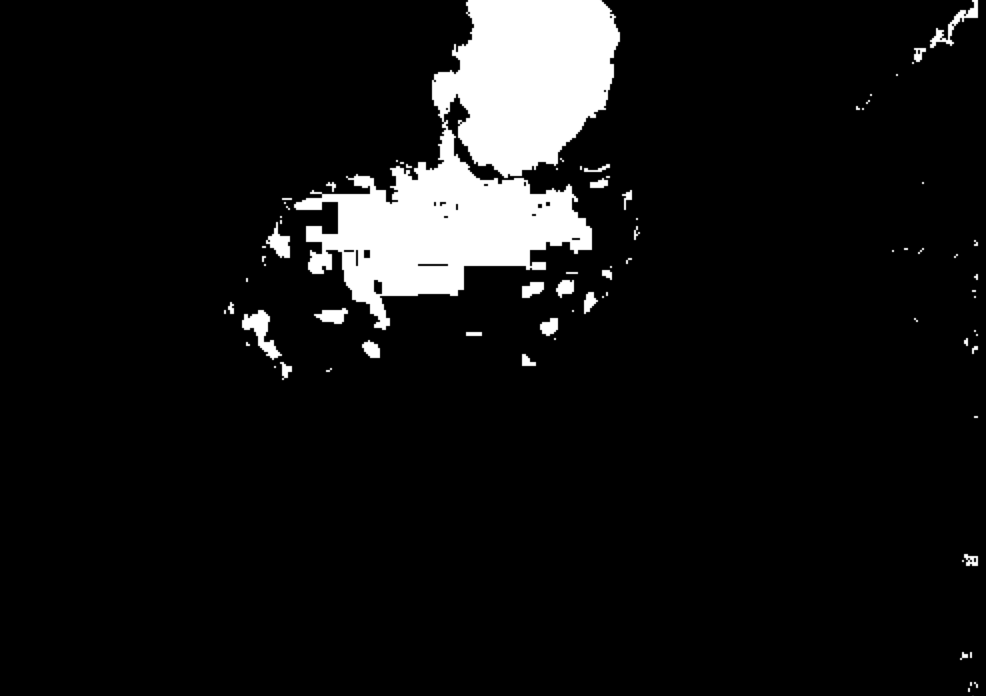
\includegraphics[width=\textwidth]{obrazky/spajanieKonturMaska}
    \caption{Roztireštená binárna maska}
  \end{minipage}
  \hfill
  \begin{minipage}[b]{0.4\textwidth}
    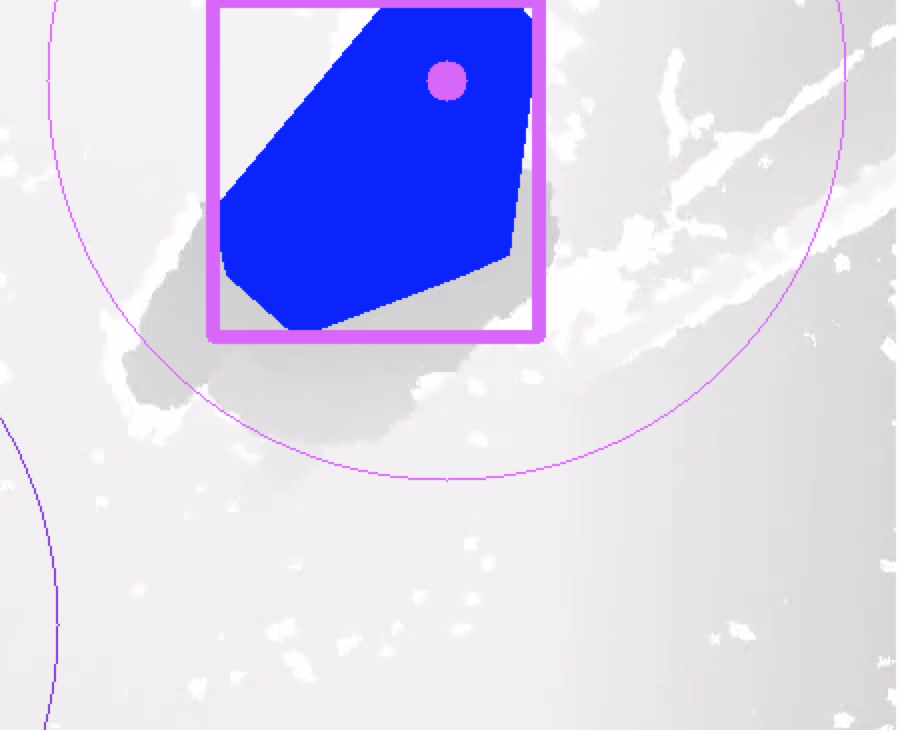
\includegraphics[width=\textwidth]{obrazky/spajanieKonturVysledok}
    \caption{Spojená kontúra}
  \end{minipage}
\end{figure}


Popis algoritmu pričom všetky kontúry nájdené prostredníctvom funkcie metódy sledovania hraníc sú uložené v zozname \textit{allCont}:
\begin{enumerate}
  \item Zo zoznamu \textit{allCont} odstránime všetky kontúry, ktoré majú nulový obsah
  \item Vytvoríme nový zoznam \textit{newContura}, vyberieme prvú kontúru z \textit{allCont} vložíme do zoznamu \textit{newContura} a označíme ju ako \textit{root}
  \item Zo zoznamu \textit{allCont} nájdeme všetky kontúre vyhovujúce podmienke minimálnej absolútnej vzdialenosti tažisek kontúr oproti kontúre označenej ako \textit{root}  
  \item Nájdené položky vlož do zoznamu \textit{newContura}, ostatné stanov ako nový zoznam \textit{allCont}
  \item Pre každú najdenú kontúru označk ako \textit{root} a  pokračuj bodom 3.
  \item Všetky kontúry v zozname \textit{newContura} spoj do jednej kontúry
  \item Pre každú konturu v zozname \textit{allCont} pokračuj bodom 2.
  
\end{enumerate}
Inými slovami algoritmus prechádza všetky kontúry a na základe vzdialenosti tažiskových bodov spája do jedného celku.





Spájanie zoznamu kontúr je realizovaná prostredníctvom volania funkcie  \textit{cv2.convexHull} ktorá pre množinou bodov points reprezentujúcich obrysové body oblasti nájde inú množinu bodov reprezentujúcich jej konvexný obal.

\subsubsection{Filtrácia nevyhovujúcich kontúr}  
Keďže poznáme približnú veľkosť kontúry, ktorej detekcia je cieľom záujmu všetky ostatné sú nežiaduce a je nutné ich odstrániť. Na základe tejto filtrácie sa program zbaví všetkých náhodných oblastí ktoré vznikli pôsobením šumu. Túto filtráciu je však možné použiť až po aplikovaní algoritmu pre spájanie kontúr. Je to posledná fáza segmentácie obrazu. 


\subsubsection{Výpočet najvyššieho bodu}
Vďaka tomu, že technologia snímania vytvára hĺbkovú mapu, je možne vrámci každej kontúry definovať lokálne maximum každej oblasti. Pri zvolenej koncepcii snímania bod patri do množiny bodov nachádzajúcich sa na vrchnej časti hlavy. Tento bod je významný pri sledovaní pohybu objektu. 

Proces nájdenia je definovaný postupom týchto krokov: 
\begin{enumerate}
  \item Vytvoríme prázdnu \textbf{masku} veľkosti snímaného obrazu \textit{np.zeros}
  \item Do \textbf{masky} vložíme kontúru, ktorej maximálnu oblasť chceme nájsť \textit{cv2.drawContours}
  \item Nájdeme minimálnu respektíve maximálnu hodnotu reprezentujúcu najvyžší bod kontúry  \textit{cv2.minMaxLoc(originalFrame, mask=mask)}
  \item Nájdenú hodnotu použijeme ako prahovú hodnotu a aplikujeme finkciu prahovania s globálnym prahom na originálny obraz. Výsledkom je binárna maska \textit{cv2.threshold}
  \item Medzi maskou vytvorenou v bode 2. a maskou vytvorenou bode 4. vykonáme logickú operáciu AND, čoho výsledkom je binárna maska maximálnej oblasti skúmanej kontúry \textit{cv2.bitwise\_and(mask, thresh)}
  \item Následne môžeme znovu vyhľadať všetky uzavrené oblasti, ktoré vznikli na obraz \textit{cv2.findContours}
  \item Vyberieme kontúru s najväčším obsahom pre ktorú vyrátame ťažisko a nájdený bod prehlásime za maximálny bod oblasti
  
\end{enumerate}







\subsection{Priradenie kontúr objektom}








\subsection{Sledovanie objektu }
